 %!Figure of `Experiment Execution' flowchart
    %% Figure `Experiment Execution' flowchart
    \begin{figure*}[htb]
        \centering
        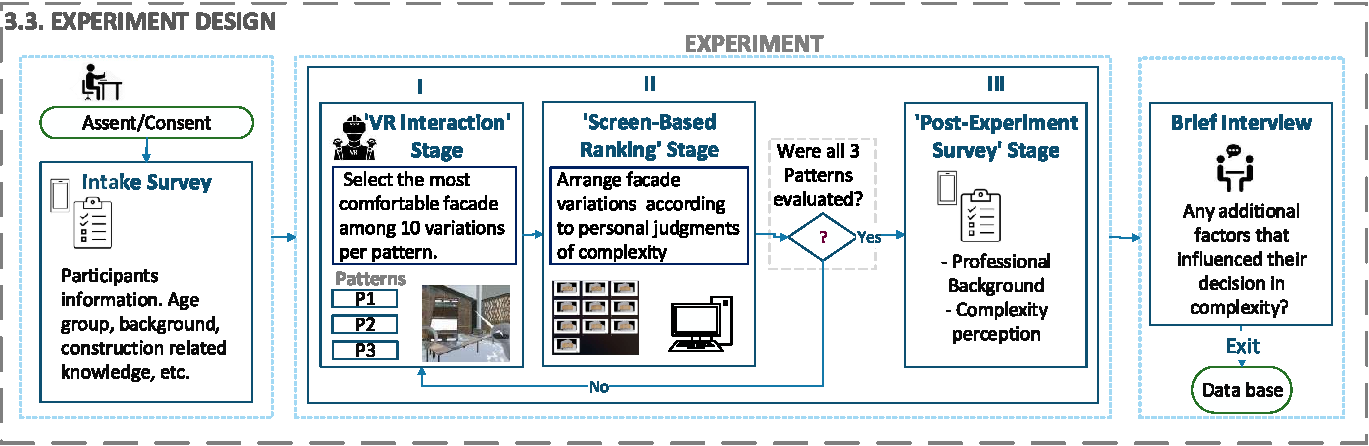
\includegraphics[width= \linewidth]{Images/FlowchartExperiment}
          \caption{`Experiment Execution' Flowchart: This flowchart outlines the three stages of the experiment, including the VR Interaction Stage (I), the Screen-Based Ranking Stage (II), and the Post-Experiment Survey (III), providing a visual representation of the sequential steps involved in the study.}
          \label{fig:ExperimentFlowchart}
    \end{figure*}

 %% CICA Flowchart
    \begin{table*}[htb]
            \centering
            \small
            \begin{tabular}{c}
                %Top cell with one figure
                %Figure Computational Image Compexity Analysis (CICA) System flowchart
                \begin{minipage}{\textwidth}
                    \centering
                    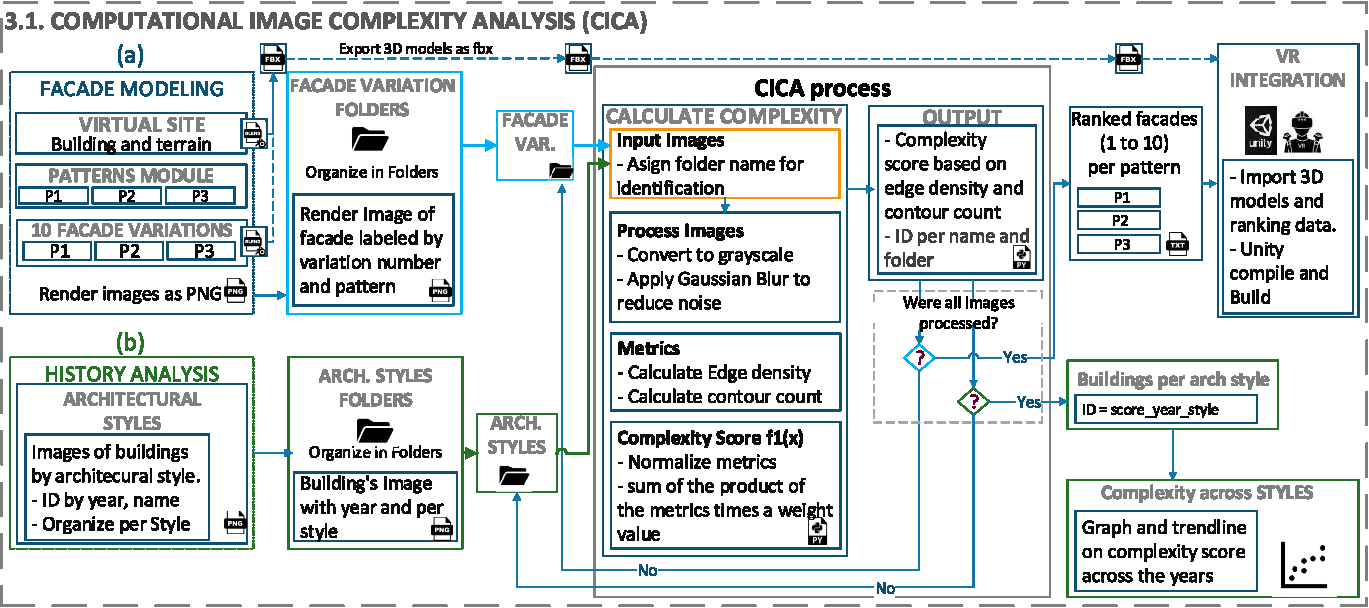
\includegraphics[width= \linewidth]{Images/CICAFlowchart}
                    \captionof{figure}{Flowchart illustrating the applications of CICA system (detailed in Section\ref{subsec:CICAsystem}), including its role in analyzing complexity scores for historical architectural styles (b) and 3D-modeled facades (a) designed with various degrees of complexity(presented in Section\ref{subsubsec:CICAfor3DmodeledFacades}).}
                    \label{fig:CICAImageEvaluationFlowchart}
                \end{minipage}
            \end{tabular}
            \end{table*}